% Created by tikzDevice version 0.12.6 on 2024-11-13 12:24:23
% !TEX encoding = UTF-8 Unicode
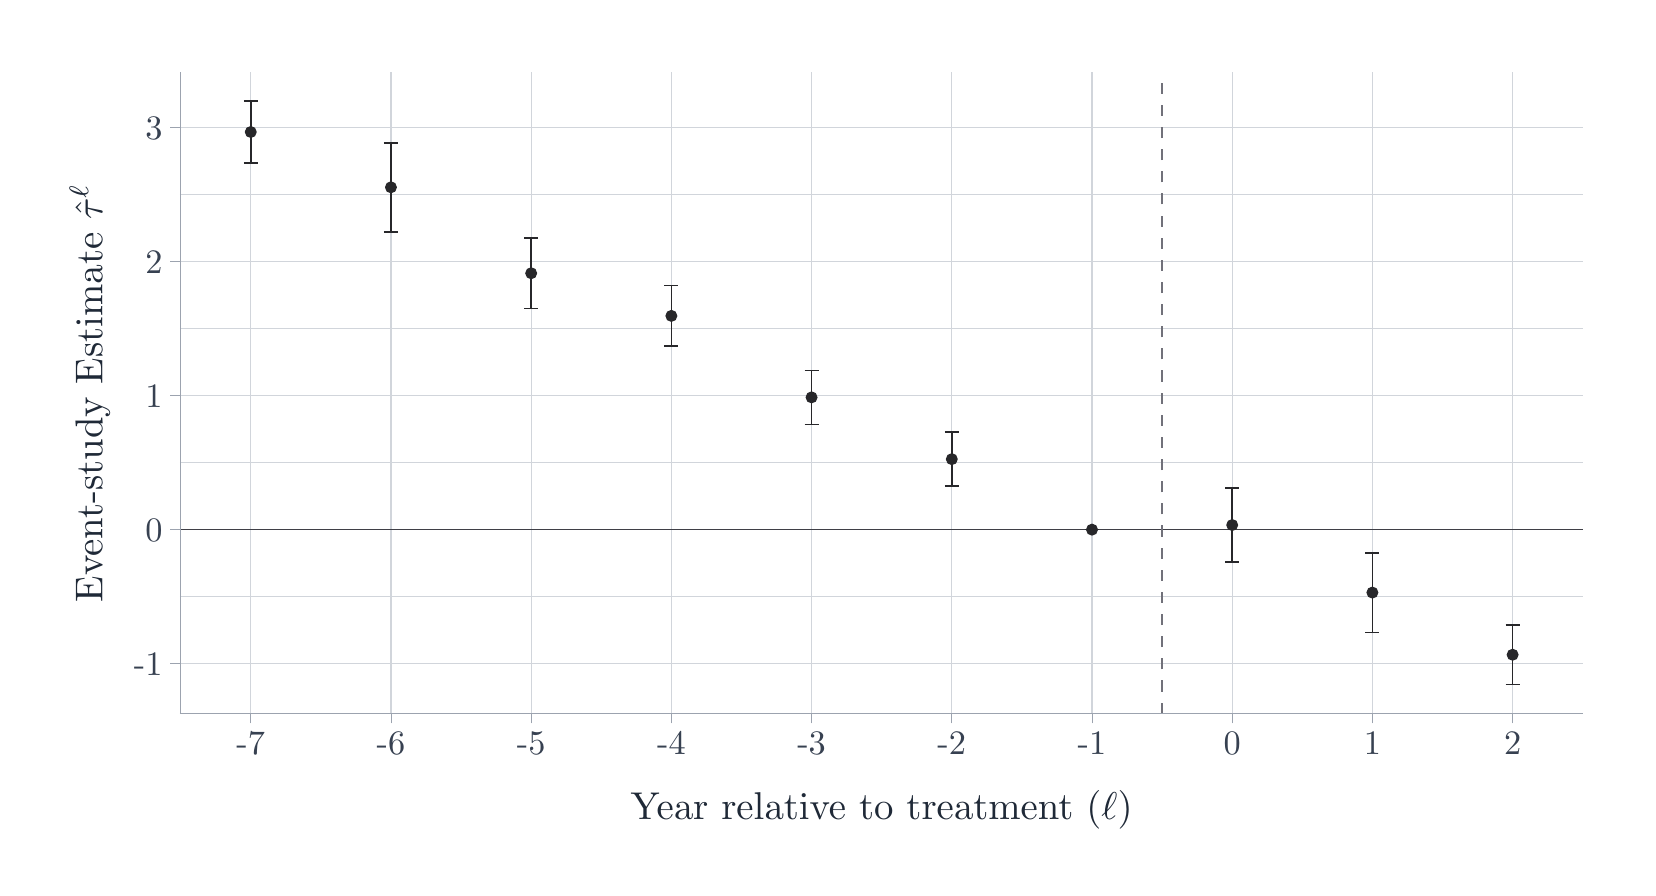
\begin{tikzpicture}[x=1pt,y=1pt]
\definecolor{fillColor}{RGB}{255,255,255}
\path[use as bounding box,fill=fillColor] (0,0) rectangle (578.16,303.53);
\begin{scope}
\path[clip] (  0.00,  0.00) rectangle (578.16,303.53);
\definecolor{drawColor}{RGB}{255,255,255}

\path[draw=drawColor,line width= 0.7pt,line join=round,line cap=round,fill=fillColor] (  0.00,  0.00) rectangle (578.16,303.53);
\end{scope}
\begin{scope}
\path[clip] ( 55.03, 55.65) rectangle (562.16,287.53);
\definecolor{drawColor}{RGB}{255,255,255}
\definecolor{fillColor}{RGB}{255,255,255}

\path[draw=drawColor,line width= 0.7pt,line join=round,line cap=round,fill=fillColor] ( 55.03, 55.65) rectangle (562.16,287.53);
\definecolor{drawColor}{RGB}{209,213,219}

\path[draw=drawColor,line width= 0.4pt,line join=round] ( 55.03, 97.92) --
	(562.16, 97.92);

\path[draw=drawColor,line width= 0.4pt,line join=round] ( 55.03,146.36) --
	(562.16,146.36);

\path[draw=drawColor,line width= 0.4pt,line join=round] ( 55.03,194.80) --
	(562.16,194.80);

\path[draw=drawColor,line width= 0.4pt,line join=round] ( 55.03,243.24) --
	(562.16,243.24);

\path[draw=drawColor,line width= 0.4pt,line join=round] ( 55.03, 73.70) --
	(562.16, 73.70);

\path[draw=drawColor,line width= 0.4pt,line join=round] ( 55.03,122.14) --
	(562.16,122.14);

\path[draw=drawColor,line width= 0.4pt,line join=round] ( 55.03,170.58) --
	(562.16,170.58);

\path[draw=drawColor,line width= 0.4pt,line join=round] ( 55.03,219.02) --
	(562.16,219.02);

\path[draw=drawColor,line width= 0.4pt,line join=round] ( 55.03,267.46) --
	(562.16,267.46);

\path[draw=drawColor,line width= 0.4pt,line join=round] ( 80.61, 55.65) --
	( 80.61,287.53);

\path[draw=drawColor,line width= 0.4pt,line join=round] (131.27, 55.65) --
	(131.27,287.53);

\path[draw=drawColor,line width= 0.4pt,line join=round] (181.94, 55.65) --
	(181.94,287.53);

\path[draw=drawColor,line width= 0.4pt,line join=round] (232.60, 55.65) --
	(232.60,287.53);

\path[draw=drawColor,line width= 0.4pt,line join=round] (283.26, 55.65) --
	(283.26,287.53);

\path[draw=drawColor,line width= 0.4pt,line join=round] (333.93, 55.65) --
	(333.93,287.53);

\path[draw=drawColor,line width= 0.4pt,line join=round] (384.59, 55.65) --
	(384.59,287.53);

\path[draw=drawColor,line width= 0.4pt,line join=round] (435.25, 55.65) --
	(435.25,287.53);

\path[draw=drawColor,line width= 0.4pt,line join=round] (485.91, 55.65) --
	(485.91,287.53);

\path[draw=drawColor,line width= 0.4pt,line join=round] (536.58, 55.65) --
	(536.58,287.53);
\definecolor{drawColor}{RGB}{63,63,70}

\path[draw=drawColor,line width= 0.6pt,line join=round] ( 55.03,122.14) -- (562.16,122.14);
\definecolor{drawColor}{RGB}{113,113,122}

\path[draw=drawColor,line width= 0.6pt,dash pattern=on 4pt off 4pt ,line join=round] (409.92, 55.65) -- (409.92,287.53);
\definecolor{drawColor}{RGB}{39,39,42}
\definecolor{fillColor}{RGB}{39,39,42}

\path[draw=drawColor,line width= 0.4pt,line join=round,line cap=round,fill=fillColor] ( 80.61,265.83) circle (  1.96);

\path[draw=drawColor,line width= 0.4pt,line join=round,line cap=round,fill=fillColor] (131.27,245.84) circle (  1.96);

\path[draw=drawColor,line width= 0.4pt,line join=round,line cap=round,fill=fillColor] (181.94,214.79) circle (  1.96);

\path[draw=drawColor,line width= 0.4pt,line join=round,line cap=round,fill=fillColor] (232.60,199.38) circle (  1.96);

\path[draw=drawColor,line width= 0.4pt,line join=round,line cap=round,fill=fillColor] (283.26,169.94) circle (  1.96);

\path[draw=drawColor,line width= 0.4pt,line join=round,line cap=round,fill=fillColor] (333.93,147.61) circle (  1.96);

\path[draw=drawColor,line width= 0.4pt,line join=round,line cap=round,fill=fillColor] (384.59,122.14) circle (  1.96);

\path[draw=drawColor,line width= 0.4pt,line join=round,line cap=round,fill=fillColor] (435.25,123.80) circle (  1.96);

\path[draw=drawColor,line width= 0.4pt,line join=round,line cap=round,fill=fillColor] (485.91, 99.40) circle (  1.96);

\path[draw=drawColor,line width= 0.4pt,line join=round,line cap=round,fill=fillColor] (536.58, 76.94) circle (  1.96);

\path[draw=drawColor,line width= 0.6pt,line join=round] ( 78.08,276.99) --
	( 83.15,276.99);

\path[draw=drawColor,line width= 0.6pt,line join=round] ( 80.61,276.99) --
	( 80.61,254.66);

\path[draw=drawColor,line width= 0.6pt,line join=round] ( 78.08,254.66) --
	( 83.15,254.66);

\path[draw=drawColor,line width= 0.6pt,line join=round] (128.74,261.91) --
	(133.81,261.91);

\path[draw=drawColor,line width= 0.6pt,line join=round] (131.27,261.91) --
	(131.27,229.76);

\path[draw=drawColor,line width= 0.6pt,line join=round] (128.74,229.76) --
	(133.81,229.76);

\path[draw=drawColor,line width= 0.6pt,line join=round] (179.40,227.54) --
	(184.47,227.54);

\path[draw=drawColor,line width= 0.6pt,line join=round] (181.94,227.54) --
	(181.94,202.05);

\path[draw=drawColor,line width= 0.6pt,line join=round] (179.40,202.05) --
	(184.47,202.05);

\path[draw=drawColor,line width= 0.6pt,line join=round] (230.07,210.30) --
	(235.13,210.30);

\path[draw=drawColor,line width= 0.6pt,line join=round] (232.60,210.30) --
	(232.60,188.46);

\path[draw=drawColor,line width= 0.6pt,line join=round] (230.07,188.46) --
	(235.13,188.46);

\path[draw=drawColor,line width= 0.6pt,line join=round] (280.73,179.69) --
	(285.80,179.69);

\path[draw=drawColor,line width= 0.6pt,line join=round] (283.26,179.69) --
	(283.26,160.19);

\path[draw=drawColor,line width= 0.6pt,line join=round] (280.73,160.19) --
	(285.80,160.19);

\path[draw=drawColor,line width= 0.6pt,line join=round] (331.39,157.35) --
	(336.46,157.35);

\path[draw=drawColor,line width= 0.6pt,line join=round] (333.93,157.35) --
	(333.93,137.86);

\path[draw=drawColor,line width= 0.6pt,line join=round] (331.39,137.86) --
	(336.46,137.86);

\path[draw=drawColor,line width= 0.6pt,line join=round] (382.05,122.14) --
	(387.12,122.14);

\path[draw=drawColor,line width= 0.6pt,line join=round] (384.59,122.14) --
	(384.59,122.14);

\path[draw=drawColor,line width= 0.6pt,line join=round] (382.05,122.14) --
	(387.12,122.14);

\path[draw=drawColor,line width= 0.6pt,line join=round] (432.72,137.11) --
	(437.78,137.11);

\path[draw=drawColor,line width= 0.6pt,line join=round] (435.25,137.11) --
	(435.25,110.49);

\path[draw=drawColor,line width= 0.6pt,line join=round] (432.72,110.49) --
	(437.78,110.49);

\path[draw=drawColor,line width= 0.6pt,line join=round] (483.38,113.80) --
	(488.45,113.80);

\path[draw=drawColor,line width= 0.6pt,line join=round] (485.91,113.80) --
	(485.91, 85.00);

\path[draw=drawColor,line width= 0.6pt,line join=round] (483.38, 85.00) --
	(488.45, 85.00);

\path[draw=drawColor,line width= 0.6pt,line join=round] (534.04, 87.69) --
	(539.11, 87.69);

\path[draw=drawColor,line width= 0.6pt,line join=round] (536.58, 87.69) --
	(536.58, 66.19);

\path[draw=drawColor,line width= 0.6pt,line join=round] (534.04, 66.19) --
	(539.11, 66.19);
\end{scope}
\begin{scope}
\path[clip] (  0.00,  0.00) rectangle (578.16,303.53);
\definecolor{drawColor}{RGB}{156,163,175}

\path[draw=drawColor,line width= 0.3pt,line join=round] ( 55.03, 55.65) --
	( 55.03,287.53);
\end{scope}
\begin{scope}
\path[clip] (  0.00,  0.00) rectangle (578.16,303.53);
\definecolor{drawColor}{RGB}{55,65,81}

\node[text=drawColor,anchor=base east,inner sep=0pt, outer sep=0pt, scale=  1.24] at ( 48.73, 69.41) {-1};

\node[text=drawColor,anchor=base east,inner sep=0pt, outer sep=0pt, scale=  1.24] at ( 48.73,117.85) {0};

\node[text=drawColor,anchor=base east,inner sep=0pt, outer sep=0pt, scale=  1.24] at ( 48.73,166.30) {1};

\node[text=drawColor,anchor=base east,inner sep=0pt, outer sep=0pt, scale=  1.24] at ( 48.73,214.74) {2};

\node[text=drawColor,anchor=base east,inner sep=0pt, outer sep=0pt, scale=  1.24] at ( 48.73,263.18) {3};
\end{scope}
\begin{scope}
\path[clip] (  0.00,  0.00) rectangle (578.16,303.53);
\definecolor{drawColor}{RGB}{156,163,175}

\path[draw=drawColor,line width= 0.3pt,line join=round] ( 51.53, 73.70) --
	( 55.03, 73.70);

\path[draw=drawColor,line width= 0.3pt,line join=round] ( 51.53,122.14) --
	( 55.03,122.14);

\path[draw=drawColor,line width= 0.3pt,line join=round] ( 51.53,170.58) --
	( 55.03,170.58);

\path[draw=drawColor,line width= 0.3pt,line join=round] ( 51.53,219.02) --
	( 55.03,219.02);

\path[draw=drawColor,line width= 0.3pt,line join=round] ( 51.53,267.46) --
	( 55.03,267.46);
\end{scope}
\begin{scope}
\path[clip] (  0.00,  0.00) rectangle (578.16,303.53);
\definecolor{drawColor}{RGB}{156,163,175}

\path[draw=drawColor,line width= 0.3pt,line join=round] ( 55.03, 55.65) --
	(562.16, 55.65);
\end{scope}
\begin{scope}
\path[clip] (  0.00,  0.00) rectangle (578.16,303.53);
\definecolor{drawColor}{RGB}{156,163,175}

\path[draw=drawColor,line width= 0.3pt,line join=round] ( 80.61, 52.15) --
	( 80.61, 55.65);

\path[draw=drawColor,line width= 0.3pt,line join=round] (131.27, 52.15) --
	(131.27, 55.65);

\path[draw=drawColor,line width= 0.3pt,line join=round] (181.94, 52.15) --
	(181.94, 55.65);

\path[draw=drawColor,line width= 0.3pt,line join=round] (232.60, 52.15) --
	(232.60, 55.65);

\path[draw=drawColor,line width= 0.3pt,line join=round] (283.26, 52.15) --
	(283.26, 55.65);

\path[draw=drawColor,line width= 0.3pt,line join=round] (333.93, 52.15) --
	(333.93, 55.65);

\path[draw=drawColor,line width= 0.3pt,line join=round] (384.59, 52.15) --
	(384.59, 55.65);

\path[draw=drawColor,line width= 0.3pt,line join=round] (435.25, 52.15) --
	(435.25, 55.65);

\path[draw=drawColor,line width= 0.3pt,line join=round] (485.91, 52.15) --
	(485.91, 55.65);

\path[draw=drawColor,line width= 0.3pt,line join=round] (536.58, 52.15) --
	(536.58, 55.65);
\end{scope}
\begin{scope}
\path[clip] (  0.00,  0.00) rectangle (578.16,303.53);
\definecolor{drawColor}{RGB}{55,65,81}

\node[text=drawColor,anchor=base,inner sep=0pt, outer sep=0pt, scale=  1.24] at ( 80.61, 40.78) {-7};

\node[text=drawColor,anchor=base,inner sep=0pt, outer sep=0pt, scale=  1.24] at (131.27, 40.78) {-6};

\node[text=drawColor,anchor=base,inner sep=0pt, outer sep=0pt, scale=  1.24] at (181.94, 40.78) {-5};

\node[text=drawColor,anchor=base,inner sep=0pt, outer sep=0pt, scale=  1.24] at (232.60, 40.78) {-4};

\node[text=drawColor,anchor=base,inner sep=0pt, outer sep=0pt, scale=  1.24] at (283.26, 40.78) {-3};

\node[text=drawColor,anchor=base,inner sep=0pt, outer sep=0pt, scale=  1.24] at (333.93, 40.78) {-2};

\node[text=drawColor,anchor=base,inner sep=0pt, outer sep=0pt, scale=  1.24] at (384.59, 40.78) {-1};

\node[text=drawColor,anchor=base,inner sep=0pt, outer sep=0pt, scale=  1.24] at (435.25, 40.78) {0};

\node[text=drawColor,anchor=base,inner sep=0pt, outer sep=0pt, scale=  1.24] at (485.91, 40.78) {1};

\node[text=drawColor,anchor=base,inner sep=0pt, outer sep=0pt, scale=  1.24] at (536.58, 40.78) {2};
\end{scope}
\begin{scope}
\path[clip] (  0.00,  0.00) rectangle (578.16,303.53);
\definecolor{drawColor}{RGB}{31,41,55}

\node[text=drawColor,anchor=base,inner sep=0pt, outer sep=0pt, scale=  1.40] at (308.59, 17.36) {Year relative to treatment ($\ell$)};
\end{scope}
\begin{scope}
\path[clip] (  0.00,  0.00) rectangle (578.16,303.53);
\definecolor{drawColor}{RGB}{31,41,55}

\node[text=drawColor,rotate= 90.00,anchor=base,inner sep=0pt, outer sep=0pt, scale=  1.40] at ( 27.00,171.59) {Event-study Estimate $\hat{\tau}^{\ell}$};
\end{scope}
\end{tikzpicture}
